\documentclass[conference]{IEEEtran}
\IEEEoverridecommandlockouts
% The preceding line is only needed to identify funding in the first footnote. If that is unneeded, please comment it out.
% Citations
\usepackage[style=numeric,sorting=none,citestyle=ieee]{biblatex}
\usepackage{hyperref}
\usepackage{cleveref}
\addbibresource{bib.bib}

%top and bottom rule of table
\usepackage{booktabs}

\usepackage{gensymb}
\usepackage{subcaption} % image side by side
\usepackage{caption} % image side by side

\usepackage{amsmath,amssymb,amsfonts}
\usepackage{algorithmic}
\usepackage{graphicx}
\usepackage{textcomp}
\usepackage{xcolor}
\usepackage{float}
\usepackage{siunitx} % for angle simbol
\def\BibTeX{{\rm B\kern-.05em{\sc i\kern-.025em b}\kern-.08em
    T\kern-.1667em\lower.7ex\hbox{E}\kern-.125emX}}
\usepackage[inline]{enumitem} %for inumeration in line

\usepackage{todonotes}
\usepackage{multirow}
\usepackage{booktabs}
\usepackage{threeparttable, tablefootnote}

\usepackage{hyperref}
\usepackage{cleveref}

\begin{document}

\title{Development of AlphaBot2 Gazebo simulator for RPi camera
{\footnotesize }
}

\author{\IEEEauthorblockN{Ana Rafael}
\IEEEauthorblockA{ Porto, Portugal\\
up201405377@fe.up.pt}
\and
\IEEEauthorblockN{C{\'a}ssio Santos}
\IEEEauthorblockA{
Feira de Santana, Brasil \\
sss.cassio@gmail.com}
}

\maketitle

\begin{abstract}
In recent years robots have been used as a motivational tool for teaching notions in several areas of knowledge. Despite the accessible price of such robots, the fact that these have to be acquired for several students and college resources are limited, induce a shifting of the development towards a fully virtual environment reduces these physical demands, allows for a safer testing environment. A simulator such Gazebo allows the visualisation of a model, the reproduction of physical properties and the interfacing with the Robotics Operating System (ROS) for message passing between nodes. The proposed system architecture focuses in the physical behaviours of the robot, and the camera sensor. Both the real and simulation model were tested through a line following algorithm. It was verified that the implemented ROS structure was functional either in the simulation as well as in the real robot for the robot control and camera activation. Further work in the validation and testing is tested for the assessment of the correct model performance.
\end{abstract}

\begin{IEEEkeywords}
AlphaBot2; Gazebo; Robotics Operating System (ROS);  \end{IEEEkeywords}

\section{Introduction}
Autonomous intelligent vehicles present an interesting development for the creation of self driving cars with capability to perform a number of tasks in different environments  \cite{costaAutonomousDrivingSimulator2016a}. Through the perception of the environment, with cameras and sensors for the recognition of lines in the paving, signs and lights in the air, obstacle identification and avoidance, the robot is expected to perform accordingly to the road traffic regulations \cite{haneObstacleDetectionSelfdriving2015}. 

Besides that, the use of robots for teaching purposes has proven to be a motivational tool for students to learn science, technology, engineering and mathematics (STEM). However, due to low budget for resources which limit the number of available robots in a university and the necessity of repair in case of damage the limited access to these materials may be a constraint for the development and experimenting phases. Robot simulations allow for an inexpensive and fast debugging process, experimental repeatability and easy alteration in the environment and robot dynamics, giving the possibility to experiment changes in numerous parameters without compromising the real robot \cite{yusofDevelopmentEducationalVirtual2011}. Such platforms provide a stand alone environment, resulting in no restrictions from lab hours or power management inherent to all physical systems. 
The AlphaBot 2 (represented in~\cref{fig:alphaBot2}) is a compact two wheeled robot with infrared (IR) sensors, line trackers, a RPi camera (oriented by two servo motors), a micro SC card, a 5V/2.5V USB adaptor, IR remote, and some additional components. Easily configured and with demo codes for its basic behaviours, described and available in \cite{waveshare}.
The present work aims to produce a Gazebo simulation of the AlphaBot2, test and finely tune the virtual model for verification of similar performances between the real and simulated robot specifically for the RPi camera.
The present paper starts by presenting a description of the developed robot and the implemented simplifications to it, in \cref{sec:SystStruc}. Additionally, the used world for testing and the ROS message-passing architecture is represented in order to have a fare understanding of the developed tasks.The \cref{sec:SimExp} presents the results and tested parameters; And finally \cref{sec:discussion&conclusions} outlines the main conclusions and future work.

\section{Methodologies} \label{sec:SystStruc}
This section yields a description of the developed robot's model in a 3D simulator, the implemented world, a simplification of the Portuguese autonomous driving competition and the ROS architecture.

\subsection{Design of the Robot Model} \label{subsec:Model}
For the design of the robot in the virtual world, first the main measurements for the several components were acquired and are detailed in~\cref{tab:measurements}. 

\begin{figure}[h]
\centering
\begin{minipage}{.45\linewidth}
  \centering
  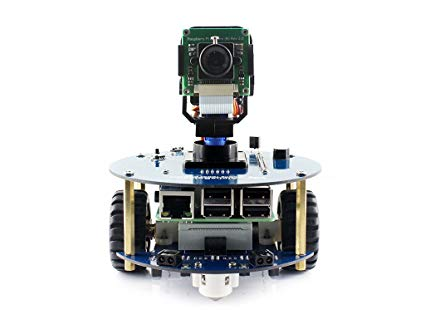
\includegraphics[width=\linewidth]{alphabot2-real.jpg}
  \captionof{figure}{AlphaBot2 front view.}
  \label{fig:alphaBot2}
\end{minipage}\quad
\begin{minipage}{.45\linewidth}
  \centering
  
\includegraphics[width=\linewidth]{floor.png}
  \captionof{figure}{Adaptation of Conde's track.}
  \label{fig:floor}
\end{minipage}\newline
\begin{minipage}{.45\linewidth}
  \centering
  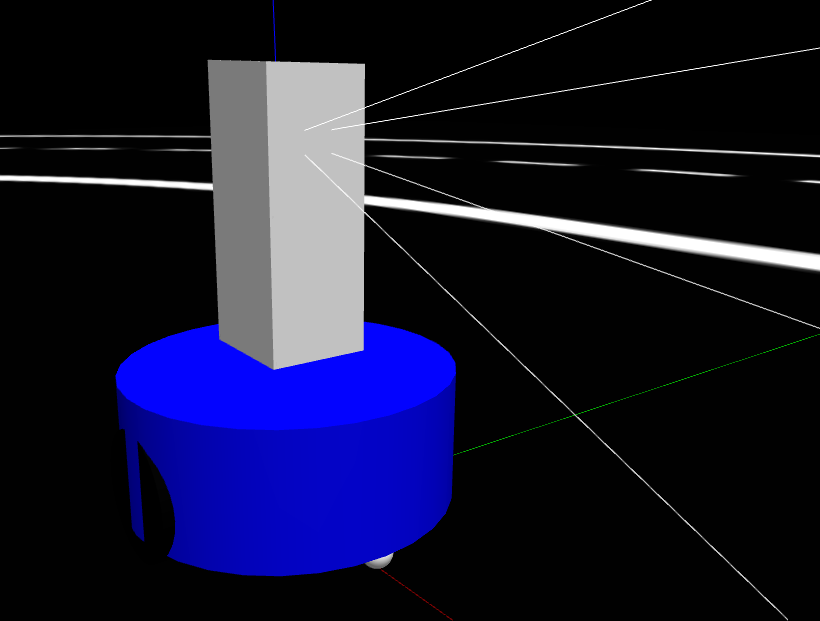
\includegraphics[width=\linewidth]{alphabot2-gazebo.png}
  \captionof{figure}{Model of the AlphaBot2 in the Gazebo simulation.}
  \label{fig:alphabot2-gazebo}
\end{minipage}\quad
\begin{minipage}{.45\linewidth}
  \centering
  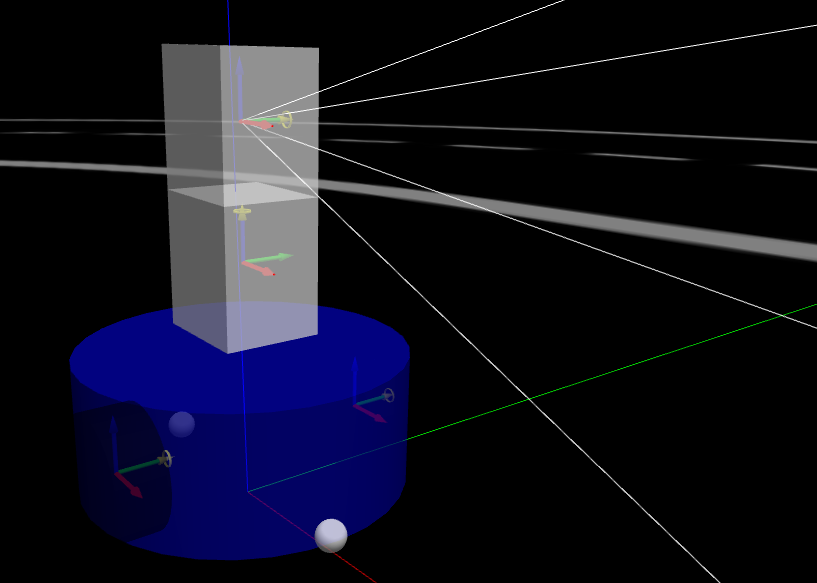
\includegraphics[width=\linewidth]{alphabot2_joints.png}
  \captionof{figure}{Visualisation of the model joints in the Gazebo simulation.}
  \label{fig:alphabot2_joints}
\end{minipage}
\end{figure}


\begin{table}[h]
\centering
\small
\begin{threeparttable}
\caption{AlphaBot 2 measurements.}
\label{tab:measurements}
\begin{tabular}{p{0.22\columnwidth}p{0.1\columnwidth}p{0.18\columnwidth}p{0.09\columnwidth}}
\toprule
\textbf{Components} & \textbf{Weight (g)} & \textbf{LWD\tnote{a}\space or DT\tnote{b} or D\tnote{c} (cm)} & \textbf{Height (cm)} \\ \midrule
Base board & 150 & \multirow{ 2}{*}{10.9x0.15} & \multirow{ 2}{*}{1.6} \\
Pi Board & 45 & &  \\
Wheels & & 4.1x1.7 & \\
Balance Wheel & & 1 & 1.5\\
Camera & 55 & 3.7x3.3x7.5 & \\
Pillars & & & 3.8 \\
Raspberry Pi & 40 & 8.4x5.5x1.7 & \\ \midrule
\textbf{Total} & & & \textbf{15.5}\\
\bottomrule
\end{tabular}
\begin{tablenotes}\footnotesize
\item [a] Length Width Depth. 
\item [b] Diameter Thickness.
\item [b] Sphere Diameter.
\end{tablenotes}
\end{threeparttable}
\end{table}
Hence, for the design of the robot in the Gazebo simulator a URDF (\textit{.xacro}) file was written. In it the links define the inertial values, collisions and visuals for each of the AlphaBot2 components. For simplification reasons the robot was designed resorting to simple shapes line cylinders and boxes, the final model is represented in~\cref{fig:alphabot2-gazebo}. Thus, the inertial values are calculated for these shapes having in consideration each of the components' weight. The joints locate the points of articulation between elements and the  plugins set the needed connections between the Gazebo simulation environment and the ROS. Since the camera orientation is controlled through two motors for pan-tilt action interfaced with the Gazebo plugin \textit{libgazebo\_ros\_control.so} and the camera is activated with the \textit{libgazebo\_ros\_camera.so}. As to the wheels these are controlled with the \textit{libgazebo\_ros\_diff\_drive.so}. A representation of the model joints is presented in~\cref{fig:alphabot2_joints}, the axis of rotation for each has a circular arrow indicating the allowed movement. 
The designed word is constituted by and adaptation of the Conde's track, as represented in~\cref{fig:floor}. 


\subsection{System architecture} \label{subsec:system_arch}
\begin{figure*}
\centering
\begin{minipage}{\linewidth}
  \centering
  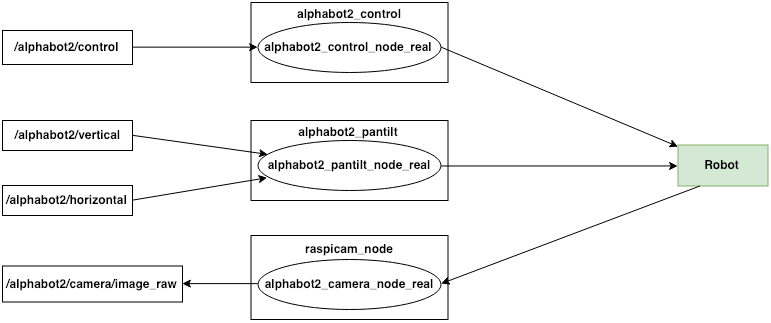
\includegraphics[width=0.7\linewidth]{arch-real.png}
  \captionof{figure}{ROS architecture for the real robot.}
  \label{fig:arch-real}
\end{minipage}\newline
\begin{minipage}{\linewidth}
  \centering
  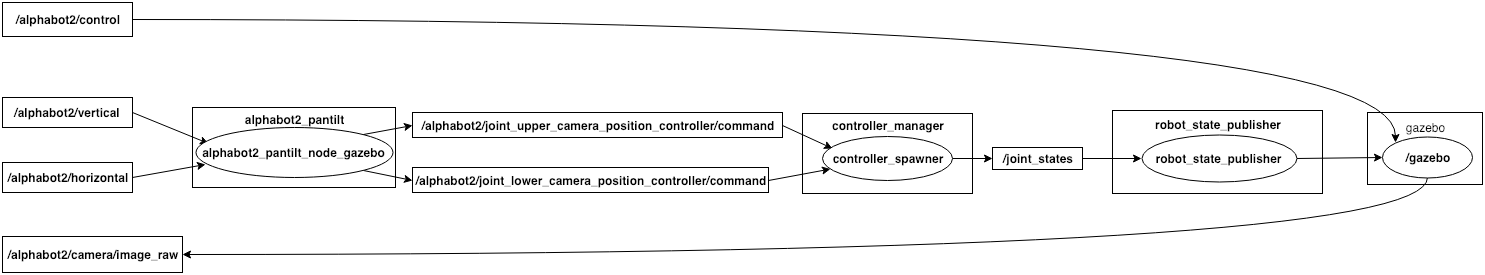
\includegraphics[width=\linewidth]{arch-gazebo.png}
  \captionof{figure}{ROS architecture for the simulator}
  \label{fig:arch-gazebo}
\end{minipage}
\end{figure*}
The system architecture is based in the ROS meta-operating system. Through the implementation of nodes which publish and subscribe to specific topics message-passing between processes is accomplished. Two levels of packages (pkg) are responsible for the control of the robots behaviour in the Gazebo simulation and in the real robot. Hence, on the side of the Gazebo simulation two nodes are implemented for the readout of the camera sensor, which publishes a raw image, and a pkg for the control of the joints present in the camera support (motions of pan and tilt), this subscribes to the angle positions for the two motors. The connections between
nodes using ROS for the real the robot are presented in \cref{fig:arch-real}, and
in \cref{fig:arch-gazebo} is shown the simulator architecture.
Using these packages, students and developers can program and test their own applications subscribing or publishing to the topics that will be described next.

\subsubsection{Ros Topics}

\begin{itemize}
    \item ``/alphabot2/control'': Publish a message of type \textit{geometry\_msgs/Twist} setting \textit{linear velocity x} and \textit{angular velocity z} to control the movement of the AlphaBot2; 
    \item ``/alphabot2/vertical'': Publish a message of type \textit{std\_msgs/Float64} setting a value between -90 and 90 to control the tilt angle of the camera;
    \item ``/alphabot2/horizonal'': Publish a message of type \textit{std\_msgs/Float64} setting a value between -90 and 90 to control the pan angle of the camera;
    \item ``/alphabot2/camera/image\_raw'': Subscribe to this topic to read a message of type \textit{sensor\_msgs/Image}.
\end{itemize}

\subsubsection{System requirements:} \label{subsec:system_requirements}
For the reuse of the system, on the side of the simulator the minimum requirements are the Ubuntu 16.04, the ROS Kinetic and the Gazebo7. As to the real robot, the used system was Raspbian GNU/LINUX 9 (stretch).

\section{Simulations and Experiments}\label{sec:SimExp}
In order to verify the correct implementation of the model and system architecture, nodes and topics, the robot was launched is an empty Gazebo's word (\cref{fig:alphaBot2_0}), and messages were published to the topics /alphabot2/vertical and /alphabot2/horizontal through the \textit{rostopic command-line tool}.

Using the command: \textit{rostopic pub /alphabot2/vertical std\_msgs/Float64 ``data: -45''} the camera starts to face the ground, represented in~\cref{fig:tilt} where it is possible to see the new position of the Tilt and its vertical axis as the dashed red line which is tilted -45 degrees. To control the Pan a std\_msgs/Float64 is published to the /alphabot2/horizontal topic using the command: \textit{rostopic pub /alphabot2/horizontal std\_msgs/Float64 ``data: -45''} (Fig \ref{fig:pan}) and \textit{rostopic pub /alphabot2/horizontal std\_msgs/Float64 ``data: 45''} (Fig \ref{fig:pan2}). It is possible to see that the camera is positioned to the right of its initial position when a negative value is submitted to the horizontal topic and it is positioned in the left if a positive value is submitted.
\begin{figure}[H]
\centering
\begin{minipage}{.45\linewidth}
  \centering
  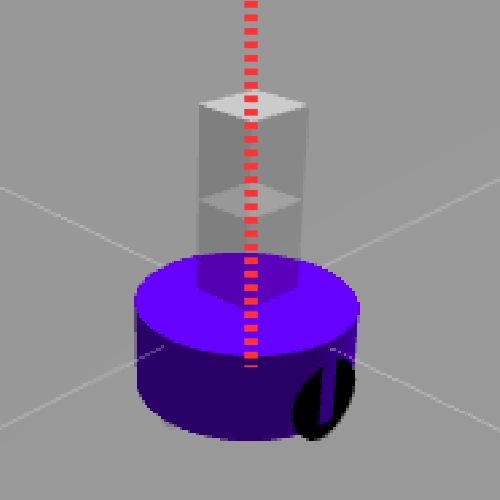
\includegraphics[width=\linewidth]{0.png}
  \captionof{figure}{Initial position}
  \label{fig:alphaBot2_0}
\end{minipage}\quad
\begin{minipage}{.45\linewidth}
  \centering
  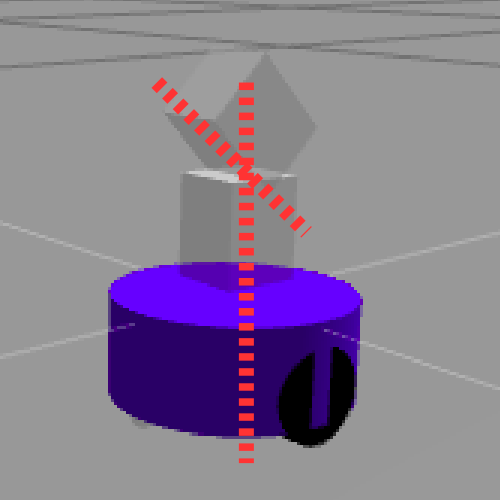
\includegraphics[width=\linewidth]{tilt.png}
  \captionof{figure}{\ang{-45} at Tilt
  }
  \label{fig:tilt}
\end{minipage}
\end{figure}
\begin{figure}[H]
\begin{minipage}{.45\linewidth}
  \centering
  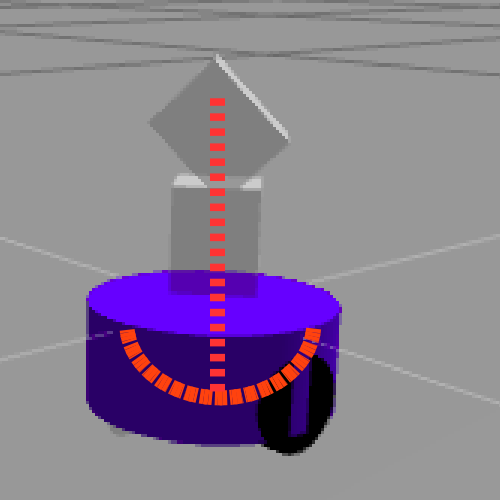
\includegraphics[width=\linewidth]{pan.png}
  \captionof{figure}{\ang{-45} at Pan}
  \label{fig:pan}
\end{minipage}\quad
\begin{minipage}{.45\linewidth}
  \centering
  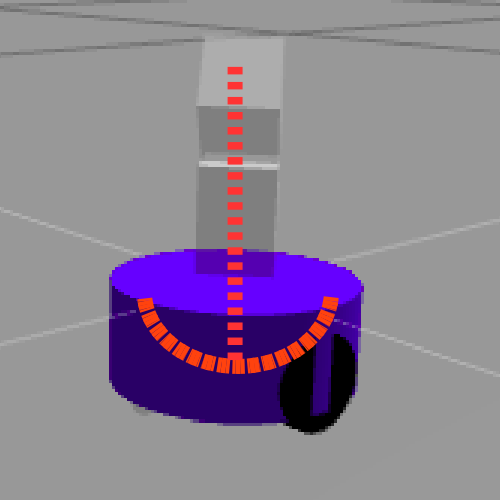
\includegraphics[width=\linewidth]{pan2.png}
  \captionof{figure}{\ang{45} at Pan}
  \label{fig:pan2}
\end{minipage}
\end{figure}

For the verification of the camera functioning in the Gazebo simulation a package called alphabot2\_tracking was created to subscribe to the /alphabot2/camera/image\_raw topic. With the robot spawned on the a world with simple objects (\cref{fig:cameraWorld}) it is possible to visualise both the RGB image captured from the camera (\cref{fig:camera}) which shows that the gazebo library is working properly for the camera sensor. On top of this node the user as freedom to operate to what best fits its needs. \cref{fig:lines} exemplifies these transformations by applying a Canny Edge Detection for future line detection using Hough Transform. This information can latter be used for the control of the robots behaviour through, for example, a PID control for the adjustment of the robot's orientation with regards to that line \cite{HTopencv}.

\begin{figure}[h]
\centering
\begin{minipage}{0.96\linewidth}
  \centering
  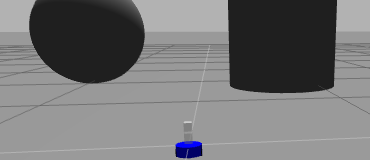
\includegraphics[width=\linewidth]{camera_world2.png}
  \captionof{figure}{Gazebo simulation with simple objects}
  \label{fig:cameraWorld}
\end{minipage}\newline
\begin{minipage}{.45\linewidth}
  \centering
  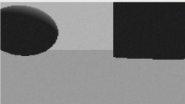
\includegraphics[width=\linewidth]{camera.png}
  \captionof{figure}{RGB image captured from the camera}
  \label{fig:camera}
\end{minipage}\quad
\begin{minipage}{.45\linewidth}
  \centering
  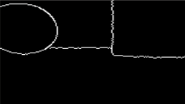
\includegraphics[width=\linewidth]{lines.png}
  \captionof{figure}{Canny Edge Detection}
  \label{fig:lines}
\end{minipage}
\end{figure}

\section{Discussion and Conclusion}\label{sec:discussion&conclusions}

In this paper it was presented a simulator and several ROS packages for the AlphaBot2 hardware abstraction and control of its low-level modules, thus allowing for a easy introduction of students to the field of robotics. The simulator was made using Gazebo as a 3D simulator and was tested by modelling the AlphaBot2 robot from Waveshare Eletronics. The simulator's components communicate with each other using the ROS framework which facilitates the user's work by suppressing concerns with low-level issues and hardware, making him only concerned with the logic behind the task. The user can then easily use the drive control of the AlphaBot2, its pantilt control and view information obtained by the camera.

The proposed objective of this paper was successfully achieved and a simulator regarding the AlphaBot2 was created. With relation to future developments improvements can be done in the \textit{.xacro} model, more specifically, more accurate representations of the robot design in the Gazebo simulation could be achieved with, for example, \textit{.stl} files for each of the components. However, these would yield superior computational requirements. 
Additionally, it is of paramount importance the evaluation of the developed model with the conduction of a comparison between the real robot and the simulated model. This can be conducted with a test setup for line following in the simulation and in the real world. Evaluating the travelled distance and the error between the relative line orientation and distance.

%\section*{References}
\printbibliography

\vspace{12pt}

\end{document}
